\chapter{A brief tour of OTB-Applications}\label{chap:otb-applications}

\section{Introduction}\label{sec:appintro}

\app was perhaps the older package of the \otb suite after the OTB
package itself. Since the \otb is a library providing remote sensing
functionalities, the only applications that were distributed at the
beginning were the examples from the Software Guide and the
tests. These applications are very useful for the developer because
their code is very short and only demonstrates one functionality at a
time, but in many cases a real application would require combining
together two or more functions from the \otb, and providing a higher
level interface to handle parameters, input and output data and
communication with the user nicely.

The \app package was originally designed to provide applications
performing simple remote sensing tasks, more complex than simple
examples from the Software Guide, and with a more user-friendly
interface (either graphical or command-line), to demonstrate the use
of the \otb functions. The most popular applications are maybe the
\application{otbImageViewerManager}, which allows to open a collection
of images and navigate in them, and the
\application{otbSupervisedClassificationApplication}, which allowed to
delineate training regions of interest on the image and classify the
image with a SVM classifier trained with these regions (this
application is no longer maintained since the same functionnality is
available through the corresponding \mont module). During the first 3
years of the \otb development, many more applications have been added
to this package, to perform various tasks. Most of them came with a
graphical user interface, apart from some small utilities that are
command-line.

The development and release of the \mont software (see
chapter~\ref{chap:Monteverdi} at the end of year 2009 changed a lot of
things for the \app package: most of non-developer users were looking
for quite a long time for an application providing \otb
functionalities under a unified graphical interface. Many applications
from the \app package were integrated to \mont as modules, and the
\app package lost a lot of its usefulness. No more applications were
added to the package and it was barely maintained, as new graphical
tools were directly embedded within \mont.

Then, some people started to regain interest in the \app
package. \mont is a great tool to perform numerous remote sensing and
image processing task in a minute, but it is not well adapted to
heavier (and longer) processing, scripting and batch
processing. Therefore, in 2010 the \app package has been revamped: old
applications have been moved to a legacy folder for backward
compatibility, and the development team started to populate the
package with compact command-line tools to perform various heavy
processing tasks. 

Later on in 2011, the \app has been further revamped. Because of the
increasing need to interface the \app into other software and to
provide auto-generated interfaces, the \otb development team decided
to develop a new application framework. The main idea of this
framework is the following: each application is written once for all
in a shared library (also known as plugin). This plugin can be
auto-loaded into appropriate tools wihtout recompiling, and is able to
fully describe its parameters, behaviour and documentation.

The tools to use the plugins can be extended, but \otb shipped the
following:
\begin{itemize}
\item A command-line laucher, which is almost equivalent to the former
  \app command-line interface,
\item A graphical launcher, with an auto-generated QT interface,
  providing ergonomic parameters setting, display of documentation,
  and progress reporting,
\item A C and SWIG interface, which means that any application can be
  loaded set-up and executed into a high-level language such as Python
  for instance.
\end{itemize}

Additionally, \href{http://www.qgis.org/}{QGis} plugins built on top of the SWIG/Python interface
are available with seamless integration within QGis.

To facilitate the use of these tools and applications, they will now
be shipped with the standard \otb package. It means that the former
\textbf{OTB-Applications} package will no longer be maintained.

The \app are now rich of more than 40 tools, which are listed in the
the applications reference documentation, presented in
chapter~\ref{chap:apprefdoc}, page~\pageref{chap:apprefdoc}.

\section{Installation}\label{sec:appinstall}

Since \app are now included within the standard \otb package, their 
installation is made while installing the whole \otb. Detailed 
instructions on how to install the whole \otb suite either from 
binary packages or from source are available in the \sg. 

Here, we will focus only on the installation of the old OTB-Applications 
package, although this package is deprecated.

\subsection{Windows 2000/XP/Vista/Seven}
\label{ssec:app_windows_binaries}

For Windows 2000/XP/Vista/Seven users, an installation program exists
for OTB-Applications. This installer depends on dependencies that can
be installed through \osgeow. The packages that need to be installed
are \emph{gdal, curl, libtiff, libgeotiff, libjpeg, zlib and libpng}.

Remember that the corresponding dlls are to be accessible in the
system path. To ensure so, add the \osgeow bin directory to your
system path.

 Once the dependencies have been properly installed, please go the the
 \download, to get the installer. Double-click on the installer and
 let it guide you through the installation process.

\subsection{MacOS X}
\label{ssec:mac_binaries}

For now, no binary package is available for OTB-Applications on 
MacOS X. You can build the OTB-Applications from sources by 
following instructions in the \sg.

\subsection{Linux}

\subsubsection{Ubuntu 10.04, 10.10 and 11.04}
\label{ssec:ubuntu_binaries}
For Unbuntu 10.04 (Lucid Lynx), 10.10 (Maverick Meerkat) and 11.04
(Natty Narwhal), the whole \otb suite is available through APT repositories.

If you are using apt command-line tools, use these command-lines to
add the otb repository to apt sources:
\begin{verbatim}
sudo aptitude install add-apt-repository 
sudo add-apt-repository ppa:otb/orfeotoolbox-stable
\end{verbatim}
Now run:
\begin{verbatim}
sudo aptitude update
sudo aptitude install otbapp
\end{verbatim}

If you are using \emph{Synaptic}, you can add the repositories, update
and install the packages through the graphical interface.

If you want to use OTB with bleeding edge versions of gdal and qgis,
there is an alternate UbuntuGIS repository.  You can add it by using
these command-lines:
\begin{verbatim}
sudo aptitude install add-apt-repository 
sudo apt-add-repository ppa:ubuntugis/ubuntugis-unstable
sudo add-apt-repository ppa:otb/orfeotoolbox-stable-ubuntugis
\end{verbatim}
Now run:
\begin{verbatim}
sudo aptitude update
sudo aptitude install otbapp
\end{verbatim}

Be careful not to add the two repositories, since they may cause
incompatibilities.

For further informations about ubuntu packages go to
\href{https://launchpad.net/~otb/+archive/orfeotoolbox-stable}{orfeotoolbox-stable
  launchpad page} and click on \textbf{Read about installing}.

\textbf{apt-add-repository} will try to retrieve the GPG keys of the
repositories to certify the origin of the packages. If you are behind
a http proxy, this step won't work and apt-add-repository will stall
and eventually quit. You can temporarily ignore this error and proceed
with the update step. Following this, aptitude update will issue a
warning about a signature problem. This warning won't prevent you from
installing the packages.

\subsubsection{OpenSuse 11.2 and higher}
\label{ssec:opensuse_binaries}

For OpenSuse 11.2 and higher, the whole \otb suite is available
through \emph{zypper}.

First, you need to add the appropriate repositories with these
command-lines (please replace $11.4$ by your OpenSuse version):
\begin{verbatim}
sudo zypper ar 
http://download.opensuse.org/repositories/games/openSUSE_11.4/ Games
sudo zypper ar 
http://download.opensuse.org/repositories/Application:/Geo/openSUSE_11.4/ GEO
sudo zypper ar 
http://download.opensuse.org/repositories/home:/tzotsos/openSUSE_11.4/ tzotsos
\end{verbatim}

Now run:
\begin{verbatim}
sudo zypper refresh
sudo zypper install Orfeo-Applications
\end{verbatim}

Alternatively you can use the One-Click Installer from the
\href{http://software.opensuse.org/search?q=Orfeo&baseproject=openSUSE\%3A11.4&lang=en&include_home=true&exclude_debug=true}{openSUSE
  Download page} or add the above repositories and install through
Yast Package Management.

In case you wish to test the latest version of the packages, you can run:
\begin{verbatim}
sudo zypper refresh
sudo zypper install Orfeo-Applications-beta
\end{verbatim}


\section{Using the applications}\label{sec:usingapps}

Using the new \app framework is slightly more complex than launching a
command-line tool. This section describes all the ways to access the
new applications. Apart from the simplified access, which is similar
to the former access to \app, to be able to launch an application, you
will need to know the application name and optionally the path where the
applications plugins are stored. For applications shipped with \otb,
the application name of each application can be found in
chapter~\ref{chap:apprefdoc}, page~\pageref{chap:apprefdoc}.

\subsection{Simplified use}

All standard applications delivered in with \otb comes with simplified
scripts in the system path, allowing to launch the command-line and QT
versions of the application the same simple way we used to launch the
old applications. The command-line interface is prefixed by
\verb?otbcli_?, while the Qt interface is prefixed by
\verb?otbgui_?. For instance, calling \verb?otbcli_Convert? will
launch the command-line interface of the \textbf{Convert} application,
while \verb?otbgui_Convert? will launch the Qt one.

For windows users, the simplified Qt interface launcher is also
available from the Start Menu.

Passing arguments to the command-line version (prefixed by
\verb?otbcli_?) is explained in next sub-section.

\subsection{Using the command-line launcher}

The command-line application launcher allows to load an application
plugin, to set its parameters, and execute it using the command
line. Launching the \verb?otbApplicationLauncherCommandLine?
without argument results in the following help to be displayed:

\begin{verbatim}
$ otbApplicationLauncherCommandLine 
Usage : ./otbApplicationLauncherCommandLine module_name [MODULEPATH] [arguments]
\end{verbatim} 

The \verb?module_name? parameter corresponds to the application
identifier. The \verb?[MODULEPATH]? argument is optional and allows 
to pass to the launcher a path where the shared library (or plugin) from
application corresponding to \verb?module_name? is. If no
\verb?[MODULEPATH]?, the launcher will look into standard \otb
installation path. An error in the application name (i.e. in parameter
\verb?module_name?) will make the
\verb?otbApplicationLauncherCommandLine? lists the name of all
applications found in \verb?[MODULEPATH]?, or in the standard \otb
installation path if \verb?[MODULEPATH]? is not provided.

Launching the \verb?otbApplicationLauncherCommandLine? with a valid
application id and no or incomplete parameters results will make the
launcher display a summary of the parameters, indicating which ones
are missing to allow for application execution. Here is an example
with the \textbf{OrthoRectification} application:

\begin{scriptsize}
\begin{verbatim}
./otbApplicationLauncherCommandLine OrthoRectification

ERROR: Waiting for at least one parameter...

====================== HELP CONTEXT ======================
NAME: OrthoRectification
DESCRIPTION: This application allows to ortho-rectify optical images from supported sensors.

EXAMPLE OF USE: 
otbcli_OrthoRectification -io.in QB_TOULOUSE_MUL_Extract_500_500.tif -io.out QB_Toulouse_ortho.tif

DOCUMENTATION: http://www.orfeo-toolbox.org/Applications/OrthoRectification.html
======================= PARAMETERS =======================
        -progress                        <boolean>        Report progress 
MISSING -io.in                           <string>         Input Image 
MISSING -io.out                          <string> [pixel] Output Image  [pixel=uint8/int8/uint16/int16/uint32/int32/float/double]
        -map                             <string>         Output Map Projection [utm/lambert2/lambert93/transmercator/wgs/epsg]
MISSING -map.utm.zone                    <int32>          Zone number 
        -map.utm.northhem                <boolean>        Northern Hemisphere 
        -map.transmercator.falseeasting  <float>          False easting 
        -map.transmercator.falsenorthing <float>          False northing 
        -map.transmercator.scale         <float>          Scale factor 
        -map.epsg.code                   <int32>          EPSG Code 
        -outputs.mode                    <string>         Parameters estimation modes [auto/autosize/autospacing]
MISSING -outputs.ulx                     <float>          Upper Left X 
MISSING -outputs.uly                     <float>          Upper Left Y 
MISSING -outputs.sizex                   <int32>          Size X 
MISSING -outputs.sizey                   <int32>          Size Y 
MISSING -outputs.spacingx                <float>          Pixel Size X 
MISSING -outputs.spacingy                <float>          Pixel Size Y 
        -outputs.isotropic               <boolean>        Force isotropic spacing by default 
        -elev                            <string>         Elevation management [dem/average]
MISSING -elev.dem.path                   <string>         DEM directory 
        -elev.dem.geoid                  <string>         Geoid File 
        -elev.average.value              <float>          Average Elevation 
        -interpolator                    <string>         Interpolation [nn/linear/bco]
        -interpolator.bco.radius         <int32>          Radius for bicubic interpolation 
        -opt.rpc                         <int32>          RPC modeling (points per axis) 
        -opt.ram                         <int32>          Available memory for processing (in MB) 
        -opt.gridspacing                 <float>          Resampling grid spacing 
\end{verbatim}
\end{scriptsize}

For a detailed description of the application behaviour and
parameters, please look for the corresponding application in the
application reference documentation presented
chapter~\ref{chap:apprefdoc}, page~\pageref{chap:apprefdoc} or
following the \verb?DOCUMENTATION? hyperlink provided in
\verb?otbApplicationLauncherCommandLine? output. Parameters are passed
to the application using the parameter key (which might include one or
several \verb?.? character), prefixed by a \verb?-?. Command-line
examples are provided in chapter~\ref{chap:apprefdoc},
page~\pageref{chap:apprefdoc}.

\subsection{Using the Qt launcher}
The Qt interface for the applications provides a usefull graphical interface
to set the parameters, choose files, and monitor the execution progress. 
This interface can be activated through the CMake option \code{WRAP\_QT} 
(it enables the build of the Qt application launcher). This launcher 
only needs the same two arguments as the command line:
\begin{verbatim}
$ otbApplicationLauncherQt module_name [MODULEPATH]
\end{verbatim}

It displays a window with several tabs:
\begin{itemize}
\item \textbf{[Parameters]} is where you set the parameters and 
execute the application. 
\item \textbf{[Logs]} is where you see the informations given by 
the application during its execution. 
\item \textbf{[Progress]} is where you see a progress bar of the 
execution (not available for all applications). 
\item \textbf{[Documentation]} is where you find a summary of the 
application documentation.
\end{itemize}

In this interface, every optional parameter has a check box that
you have to tick if you want to set a value and use this parameter.
The mandatory parameters cannot be unchecked.
 
The Qt interface of the application \application{Rescale} is shown 
here as an example.

\begin{figure}[h]
  \center
  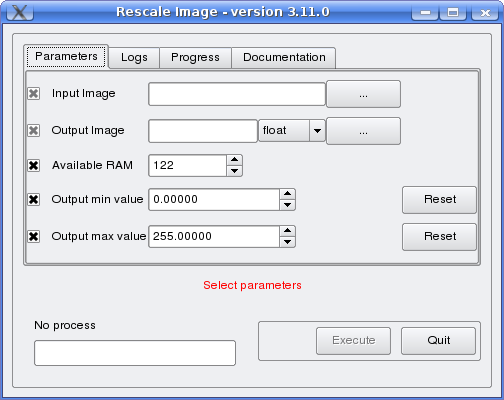
\includegraphics[width=0.6\textwidth]{../Art/QtImages/rescale_param.png}
  \itkcaption[GUI of the application Rescale, parameters tab]{Parameters tab in \application{Rescale} application.}
  \label{fig:rescaleParam}
\end{figure}

\begin{figure}[h]
  \center
  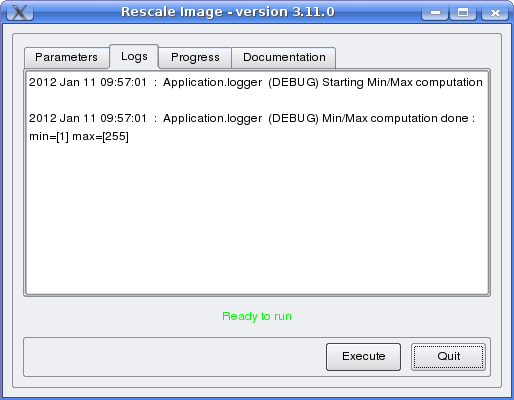
\includegraphics[width=0.6\textwidth]{../Art/QtImages/rescale_logs.png}
  \itkcaption[GUI of the application Rescale, logs tab]{Logs tab in \application{Rescale} application.}
  \label{fig:rescaleLogs}
\end{figure}

\begin{figure}[h]
  \center
  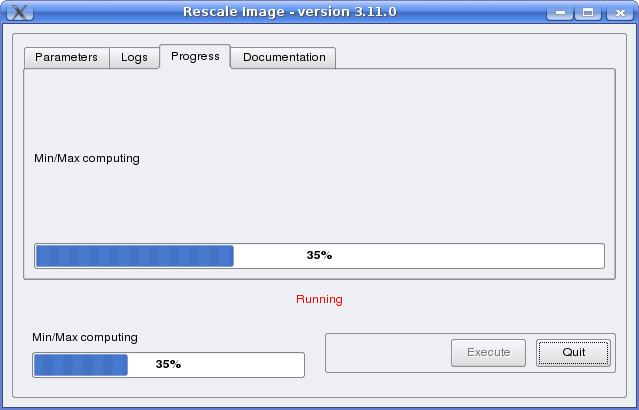
\includegraphics[width=0.6\textwidth]{../Art/QtImages/rescale_progress.png}
  \itkcaption[GUI of the application Rescale, progress tab]{Progress tab in \application{Rescale} application.}
  \label{fig:rescaleProgress}
\end{figure}

\begin{figure}[h]
  \center
  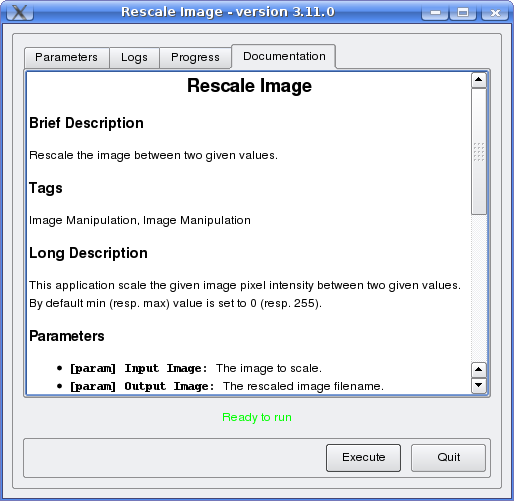
\includegraphics[width=0.6\textwidth]{../Art/QtImages/rescale_documentation.png}
  \itkcaption[GUI of the application Rescale, parameters tab]{Parameters tab in \application{Rescale} application.}
  \label{fig:rescaleDocumentation}
\end{figure}

\subsection{Using the SWIG interface}

